\section{Introduction et Contexte du Problème}

Le sujet porte sur la planification des prises de vue du satellite d'observation optique SPOT-5. Ce problème consiste à décider, pour chaque journée, quelles images seront acquises le lendemain et par quel instrument, à partir d'un ensemble de commandes de clients du monde entier.

\subsection{Caractéristiques Orbitales et Instruments}
D'après les spécifications fournies :
\begin{itemize}
    \item Orbite : circulaire (altitude constante de l'ordre de $700\text{ km}$), quasi-polaire et héliosynchrone, décrivant environ 14 révolutions de $100\text{ minutes}$ par jour avec un cycle de 25 jours. Les prises de vue optiques sont réalisées exclusivement de jour, lors de la descente du pôle Nord vers le pôle Sud.
    \item Instruments d'observation : le satellite embarque trois instruments optiques identiques équipés chacun d'un miroir de visée indépendant orientable latéralement, couvrant un corridor au sol de $800\text{ km}$ de large ($400\text{ km}$ de chaque côté de la trace) :
    \begin{itemize}
        \item Instrument 1 (Avant) : pointeur incliné vers l'avant dans le plan orbital (angle fixe d'environ $+25^\circ$).
        \item Instrument 2 (Nadir / Centre) : pointeur vertical vers le centre de la Terre ($0^\circ$).
        \item Instrument 3 (Arrière) : pointeur incliné vers l'arrière dans le plan orbital (angle fixe d'environ $-25^\circ$).
    \end{itemize}
    \item Images cibles : chaque commande correspond à une zone carrée d'environ $60\text{ km}$ de côté.
\end{itemize}

\begin{figure}[H]
    \centering
    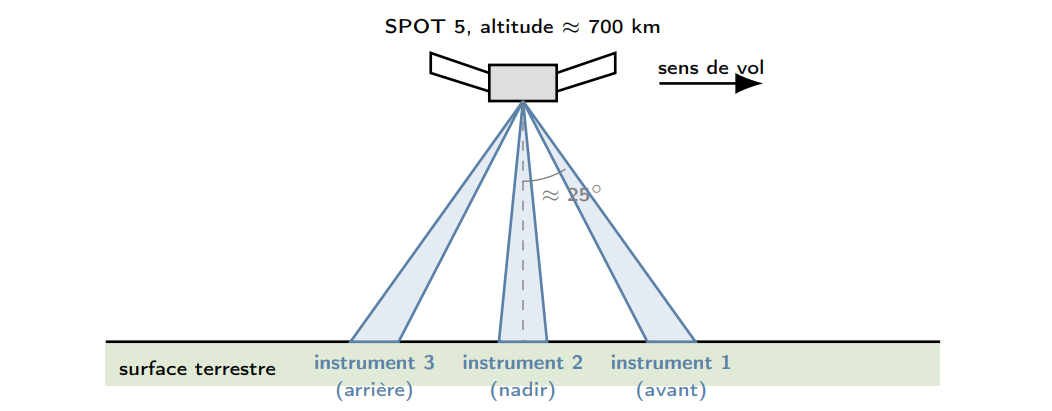
\includegraphics[width=0.78\textwidth]{spot_geometry.png}
    \caption{Disposition des trois instruments optiques de SPOT-5 le long de l'orbite (source : support de cours version slides).}
    \label{fig:spot_schema}
\end{figure}

\subsection{Types de Prises de Vue et Contraintes du Sujet}
Deux types de demandes coexistent :
\begin{itemize}
    \item Images monoscopiques ($TY=1$) : Une seule acquisition, réalisable par n'importe lequel des trois instruments.
    \item Images stéréoscopiques ($TY=2$) : Deux images acquises au cours de la même révolution pour restituer le relief, requérant obligatoirement les instruments 1 (avant) et 3 (arrière), sans utiliser l'instrument 2.
\end{itemize}

La planification doit respecter les contraintes physiques et technologiques définies dans l'énoncé :
\begin{itemize}
    \item Capacité mémoire : La quantité totale de mémoire $PM$ stockée à bord ne doit pas dépasser la capacité maximale $PM_{\max}$ du satellite (la mémoire requise est déjà doublée pour les stéréos dans les données).
    \item Non-chevauchement temporel et dépointage : Deux images programmées sur un même instrument ne peuvent pas se chevaucher et doivent laisser un délai suffisant pour la rotation angulaire du miroir à la vitesse $V_I$.
    \item Incertitudes : Les images nuageuses ne sont pas vendues (intervalle de probabilité de nuages $[ProbaInf, ProbaSup]$). De plus, chaque instrument présente une probabilité de défaillance ($Failure$).
\end{itemize}
